\chapter{Elastyczne indeksowanie}

Termin ,,elastyczne indeksowanie'' (\emph{flexible indexing}) określa nowe podejście do architektury Lucene, wprowadzone w wersji 4.0. Polega ono na oddzieleniu formatu indeksu (fizycznego sposobu zapisu poszczególnych jego elementów na dysku) od logicznych operacji na nim wykonywanych.

\section{Cel wprowadzenia zmian}

W październiku 2012 roku, po ok. dwóch latach prac, została opublikowana wersja 4.0 Lucene, znacząco różniąca się od poprzednich -- głównie dzięki wprowadzeniu tzw. \emph{architektury kodekowej}. Części biblioteki odpowiedzialne za indeksowanie zostały logicznie wydzielone i umieszczone w dodatkowej warstwie architektury (kodeku). 

Głównym powodem wprowadzenia zmian był przestarzały i nieelastyczny format kodowania indeksu. Wersje 3.x Lucene oraz wcześniejsze do zapisu list postingowych posługiwały się formatem \texttt{vInt} -- liczb całkowitych o zmiennej liczbie bajtów. Format ten był ściśle związany z wszystkimi częściami kodu, w związku z czym jakakolwiek jego modyfikacja wymagała sporego nakładu pracy programisty. Utrudniało to rozwój Lucene oraz eksperymentowanie z nowymi sposobami kompresji czy strukturami danych. Format \texttt{vInt} istniał w Lucene praktycznie od jej początków (ok. 10 lat, od wersji 1.0). Od tego czasu powstały efektywniejsze algorytmy kompresji, które właśnie z powodu nieelastycznej architektury nie mogły być łatwo przetestowane.

Stara architektura uniemożliwiała także zapis dodatkowych statystyk do indeksu -- co utrudniało (lub uniemożliwiało) implementacje nowych algorytmów obliczania miar dopasowania dokumentu do zapytania.

Lucene, pomimo, że była najpopularniejszym narzędziem do wyszukiwania tekstowego stosowanym w komercyjnych projektach, rzadko była wykorzystywana w środowiskach naukowych -- właśnie ze względu na brak możliwości łatwych zmian formatów indeksu i eksperymentowania na nim. Nowa architektura miała to zmienić: umożliwić bardziej elastyczny rozwój przy jednoczesnym zachowaniu wydajności.

\section{Architektura oparta o kodeki}

Zmiany architektury polegały na wprowadzeniu dodatkowej warstwy pośredniczącej pomiędzy formatem dyskowym indeksu a biblioteką. Ilustruje to rysunek ~\ref{fig:newarchitecture} (źródło: \cite{flexindex}).

\begin{figure}[here]
 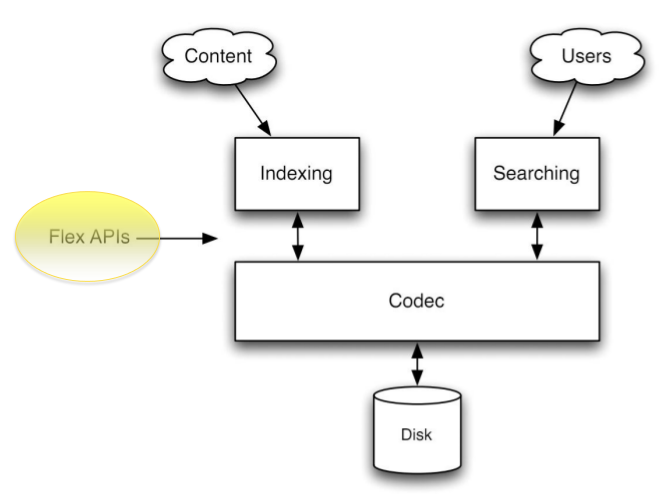
\includegraphics[scale=0.5]{pictures/architecture.png}
 \caption{Schemat architektury opartej o kodeki.\label{fig:newarchitecture}}
\end{figure}

Operacje na indeksie (dodawanie, usuwanie lub modyfikowanie dokumentów, wyszukiwanie) są implementowane w wyższych warstwach biblioteki (moduły \emph{Indexing} i \emph{Searching} na rys. \ref{fig:newarchitecture}). Kodek dostarcza formatu narzędzi do zapisu i odczytu danych o zaindeksowanych dokumentach. Poprzez jego podmianę można zastosować np. niestandardowe algorytmy kompresji, struktury danych do przechowywania słowników termów itp.

\section{Struktura kodeka}
\label{sec:codecStructure}

[Uzupełnić: kodek jest klasą o konkretnym interfejsie, ładowanie przez Java SPI.]

Aby zaimplementować własny kodek, należy przeciążyć abstrakcyjną klasę \texttt{Codec}, gromadzącą poszczególne jego elementy (tzw. formaty).

Każdy kodek składa się z ośmiu części, które luźno odpowiadają plikom zapisywanym na dysku (tzn. przyjmuje się, że każda część kodeka zapisuje i odczytuje swój plik -- nie jest to jednak konieczność). Istnieje możliwość łączenia istniejących rozwiązań z własnymi implementacjami -- można skorzystać z domyślnych implementacji większości elementów kodeka i podmienić np. tylko część odpowiedzialną za kodowanie list postingowych.

Elementy, na które składa się kodek to:
\begin{enumerate}
 \item format list postingowych (\texttt{PostingsFormat}),
 \item format DocValues (\texttt{DocValuesFormat}),
 \item format pól przechowywanych (\emph{stored fields}, \texttt{StoredFieldsFormat}),
 \item format dla \emph{term vectors} (\texttt{TermVectorsFormat}),
 \item format informacji o polach i związanych z tym statystyk (\texttt{FieldInfosFormat}),
 \item format zapisu ogólnych informacji dotyczących segmentów (\texttt{SegmentInfoFormat}),
 \item format zapisu norm (\texttt{NormsFormat}) -- związanych z poszczególnymi polami liczb wskazujących, czy dane pole powinno być traktowane jako mniej lub bardziej istotne niż pozostałe (wskaźniki \emph{boost} zapisywanie podczas indeksowania),
 \item format do zapisu informacji o tym, które dokumenty powinny zostać usunięte podczas najbliższej optymalizacji indeksu (\texttt{LiveDocsFormat}).
\end{enumerate}

\section{Czterowymiarowa struktura indeksu}

Zmiany, poza rozdzieleniem formatu zapisu indeksu do plików od architektury, dotyczyły także interfejsu programisty. Dostęp do poszczególnych elementów indeksu, czyli pól, termów, numerów dokumentów, pozycji wystąpień termu w dokumencie, itp. odbywa się przy pomocy tzw. \emph{czterowymiarowego API}, które obrazowo przedstawione jest na rys. \ref{fig:4dimAPI} (źródło: \cite{flexindex}).

\begin{figure}[here]
 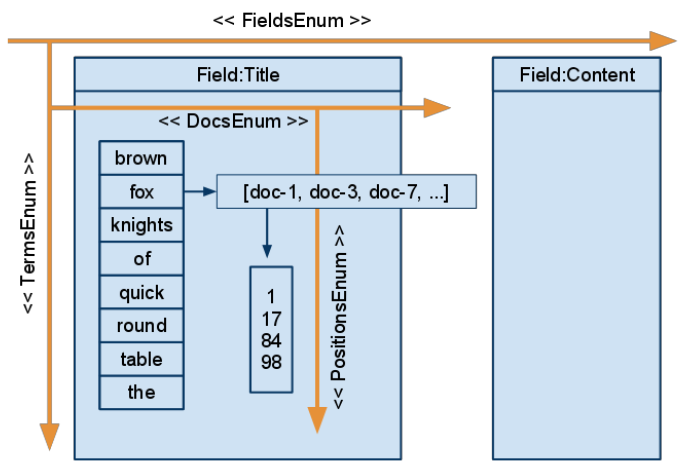
\includegraphics[scale=0.5]{pictures/api.png}
 \caption{Schemat interfejsu programisty pozwalającego na dostęp do poszczególnych elementów indeksu.\label{fig:4dimAPI}}
\end{figure}

Najbardziej nadrzędnym elementem dostępu do indeksu jest pole (\texttt{Field}). W uproszczeniu, dla każdego indeksu (bądź jego abstrakcji) możemy pobrać listę jego pól (przedstawione tutaj jako \texttt{FieldsEnum}, implementowane jako \texttt{Fields}). Pole, poza tytułem, posiada listę termów, do której mamy dostęp poprzez iterator \texttt{TermsEnum}. Dla każdego termu możemy pobrać listę dokumentów, w których on wystąpił (\texttt{DocsEnum}), a dla każego z dokumentów -- listę pozycji wystąpień (\texttt{PositionsEnum} -- jak zostanie to omówione później, w faktycznej implementacji iteratory \texttt{DocsEnum} i \texttt{PositionsEnum} są zaimplementowane jako jedna klasa).

Powyższy schemat nie oddaje faktycznej architektury dostępu do elementów indeksu -- jest jedynie jej nakreśleniem. Rysunek poniżej (\ref{fig:indexApi}) ilustruje, w jaki sposób koncepcja czterowymiarowego API została przełożona na abstrakcyjne klasy Lucene Core. [Do uzupełnienia: to jest właśnie definicja serwisu, który ma być dostarczony przez SPI] Programista chcący zaimplementować własny kodek musi stworzyć swoją hierarchię klas zgodnie z tą strukturą.

\begin{figure}[here]
 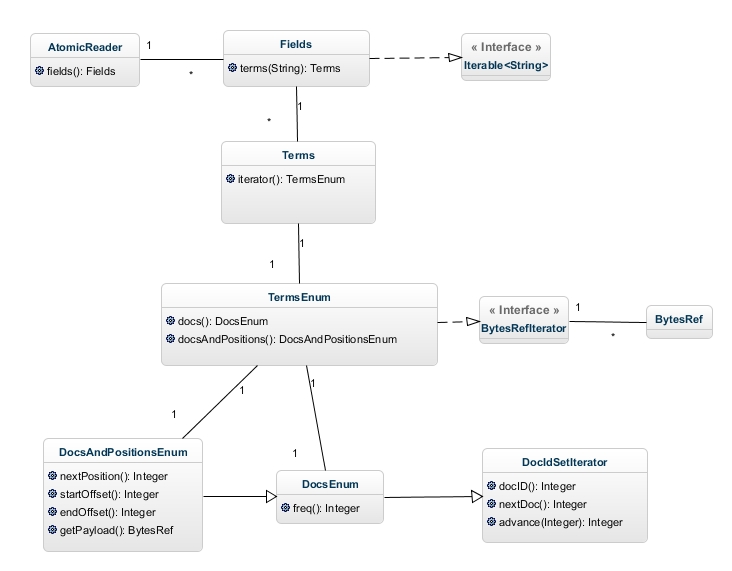
\includegraphics[scale=0.6]{pictures/LuceneAccessAPI.jpg}
 \caption{Struktura klas służących do pobierania poszczególnych elementów indeksu. Źródło: opracowanie własne.\label{fig:indexApi}}
\end{figure}

Jak zostało to wcześniej wspomniane, pola są najwyższą warstwą w hierarchii dostępu do danych indeksu. Dodatkowo, istnieje możliwość skonfigurowania, który kodek powinien być używany do zakodowania wskazanego pola. Możemy więc myśleć o indeksie zawierającym wiele pól jako o kilku równoległych indeksach. To także ma wpływ na sposób traktowania termów: ten sam term, ale znajdujący się w dwóch różnych polach jest traktowany jako dwa osobne termy. 

Zajmijmy się teraz omówieniem poszczególnych klas diagramu \ref{fig:indexApi}. \texttt{AtomicReader} jest abstrakcyjnym rozszerzeniem \texttt{IndexReadera}, który pozwala na dostęp do informacji przechowywanych w indeksie odwróconym -- w szczególności do jego pól (\texttt{IndexReader} sam w sobie nie posiada takiej funkcjonalności -- podobnie jak niektóre jego klasy potomne. Zagadnienie to jest szerzej omówione w sekcji \ref{sec:indexReader}). 

\texttt{AtomicReader} potrafi zwrócić obiekt \texttt{Fields}, implementujący interfejs iteratora napisów (\texttt{Iterable<String>}, pochodzący ze standardowej biblioteki Javy). Oznacza to, że \texttt{Fields.iterator()} przechodzi po wszystkich nazwach pól znajdujących się w indeksie. Z obiektu \texttt{Fields} można pobrać obiekt \texttt{Terms}, który poza iteratorem termów (\texttt{TermsEnum}) zawiera także statystyki dotyczące wszystkich termów pola (liczba dokumentów, w których ten term występuje, łączna liczba wystąpień termu w polu).

Od wersji 4.0 Lucene term jest reprezentowany jako ciąg bajtów (a nie, jak wcześniej, jako napis w kodowaniu UTF-16). Pozwala to na uniknięcie problemów związanych z kodowaniem znaków, szczególnie w językach wschodnioazjatyckich -- odpowiedzialność za kodowanie i odkodowywanie znaków z ciągu bajtów jest przerzucona na kodek. Klasą wykorzystaną do reprezentacji takiego ciągu jest \texttt{BytesRef} (który tak naprawdę przechowuje informacje o początku danego podciągu oraz jego długości w większej tablicy typu \texttt{byte[]}).

Zauważmy, że \texttt{TermsEnum} implementuje interfejs \texttt{BytesRefIterator}. Oznacza to tyle, że jest on w stanie wylistować wszystkie przechowywane termy. Tę samą funkcjonalność można byłoby uzyskać wykorzystując standardowy iterator dla Javy (\texttt{TermsEnum} mogłoby implementować \texttt{Iterable<BytesRef>}). Wygląda na to, że wprowadzanie dodatkowej klasy, \texttt{BytesRefIterator}, jest niepotrzebne i powoduje tylko spadek czytelności kodu.

W zależności od tego, czy podczas indeksowania dla każdego wystąpienia termu zostały zapisane dodatkowe informacje (pozycje wystąpień, \emph{payloads}), do wylistowania dokumentów, w których wystąpił dany term można użyć jednej z dwóch abstrakcji: \texttt{DocsEnum} lub rozszerzającego \texttt{DocsAndPositionsEnum}. Obydwie klasy są dostępne z poziomu obiektu \texttt{TermsEnum} -- dla termu wskazywanego obecnie przez iterator istnieje możliwość pobrania tak opakowanej listy dokumentów.

Zauważmy, że do wylistowania wszystkich dokumentów z \texttt{DocsEnum} wykorzystany jest kolejny interfejs iteratora: \texttt{DocIdSetIterator}. W tym wypadku wprowadzenie dodatkowej klasy dla tej samej funkcjonalności wydaje się jednak uzasadnione: \texttt{DocIdSetIterator}, poza standardowymi funkcjami iteratora, pozwala na przejście do wskazanego elementu listy (abstrakcyjne metody \texttt{advance(int target)} oraz \texttt{slowAdvance(int target)}: dokumentacja sugeruje, aby implementacja pierwszej z nich wykorzystywała skip listy).

\section{Dostęp do plików indeksu: \texttt{IndexReader} i jego implementacje}
\label{sec:indexReader}

Pliki indeksu w najczęstszym przypadku przechowywane są w jednym katalogu dyskowym. Nic jednak nie stoi na przeszkodzie, aby indeks był rozproszony pomiędzy wiele folderów lub maszyn lub żeby był przechowywany w pamięci RAM (takie rozwiązanie zostało już zaprezentowane w rozdziale pierszym. Stosuje się je często w celach testowych).

W przykładzie z pierwszego rozdziału przedstawiono prosty odczyt indeksu przy pomocy klas \texttt{IndexReader} i \texttt{DirectoryReader}. W tej sekcji omówione zostaną także inne sposoby dostępu do indeksu w Lucene. Schemat klas implementujących tę funkcjonalność przedstawia rys. \ref{fig:indexReader}. 

\begin{figure}[here]
 \centering
 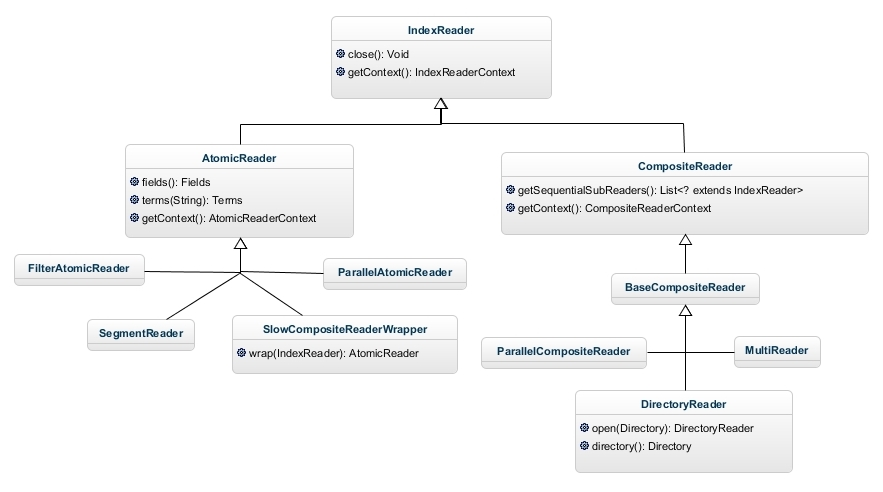
\includegraphics[scale=0.5]{pictures/Readers.jpg}
 \caption{Struktura klas dostępu do indeksu: \texttt{IndexReader} oraz klasy potomne. Źródło: opracowanie własne. \label{fig:indexReader}}
\end{figure}

Abstrakcyjny \texttt{IndexReader}, stojący na szczycie tej hierarchii, dostarcza tylko najbardziej podstawowych funkcji, wspólnych wszystkim klasom odczytującym (takich jak zamykanie indeksu -- metoda \texttt{close()}, obliczanie prostych statystyk, liczby dokumentów w indeksie, informacji o tym, czy dany indeks posiada dokumenty usunięte, itp.). 

\texttt{IndexReader} nie ma dostępu do zawartości indeksu odwróconego -- poprzez jego interfejs można uzyskać jedynie wartości pól przechowywanych. Wszystkie inne zaindeksowane informacje muszą zostać pobrane z jego rozszerzeń. Taka decyzja architektoniczna podyktowana jest chęcią uproszczenia procesu wyszukiwania z punktu widzenia programisty: użytkownik Lucene nie musi tak naprawdę nic wiedzieć o indeksie odwróconym, zaindeksowanych termach czy listach postingowych. Wystarczy, że poda bibliotece odpowiednio skonstruowane zapytanie i odbierze wyniki w postaci listy referencji do pasujących dokumentów. Wartości pól przechowywanych mogą być mu przydatne do zaprezentowania wyników. Projektanci Lucene zdecydowali, że najogólniejsza klasa dostępu do indeksu będzie posiadała ograniczone funkcjonalności.

Z \texttt{IndexReadera} wywiedzione są dwie abstrakcyjne klasy: \texttt{AtomicReader} oraz \texttt{CompositeReader}. \texttt{AtomicReader} umożliwia dostęp do indeksu na poziomie segmentu. Pozwala na pobranie informacji o indeksie odwróconym: o zaindeksowanych termach, polach, postingach, czy \emph{docValues}. Dlatego, m.in., jego implementacje (najczęściej \texttt{SegmentReader}) są niezbędne podczas łączenia segmentów i innych wewnętrznych operacji.

Ponieważ w większości przypadków indeks składa się z kilkunastu -- kilkudziesięciu segmentów, użytkownicy Lucene rzadko korzystają z implementacji \texttt{AtomicReadera} -- dużo bardziej przydatne okazuje się wykorzystanie \texttt{CompositeReaderów}, z których najbardziej popularnym jest \texttt{DirectoryReader}. Klasy wywiedzione z \texttt{CompositeReadera} nie dostarczają żadnych nowych funkcjonalności w stosunku do \texttt{IndexReadera} -- tak samo, nie pozwalają na dostęp do indeksu odwróconego. Implementują jednak dostęp do ,,łączonych indeksów'', dyskowych lub rozproszonych: agregują inne rozszerzenia klasy \texttt{IndexReader} i np. pobieranie informacji z list postingowych przekazują do odpowiednich \texttt{AtomicReaderów}. Są przykładem implementacji wzorca projektowego o nazwie kompozyt.

\texttt{CompositeReaders} pozwalają też na dostęp do swoich elementów: można je wylistować przy pomocy metody \texttt{CompositeReader.getSequentialSubReaders()} -- zatem programista chcący uzyskać np. listę termów zaindeksowanych w indeksie dyskowym ma możliwość odczytania list z poszczególnych ,,readerów atomowych''.

Innym sposobem uzyskania funkcjonalności \texttt{AtomicReadera} dla ,,readera złożonego'' jest skorzystanie z klasy \texttt{SlowCompositeReaderWrapper}, która poprzez metodę \texttt{wrap()} przyjmuje instancję \texttt{CompositeReadera} i w wyniku zwraca obiekt ,,udający'' \texttt{AtomicReader}. Wewnątrz sekwencyjnie ,,przechodzi'' po wszystkich zagregowanych \texttt{AtomicReaderach} i w locie łączy pobrane z nich dane.

\subsection{\texttt{IndexReaderContext}}

W działającym programie wykorzystującym Lucene instancje typu \texttt{IndexReader} tworzą strukturę drzewiastą, w której węzłami są implementacje klasy \texttt{CompositeReader} a liśćmi -- \texttt {AtomicReader}. Każdy element tej struktury posiada informacje o ,,swoim'' fragmencie indeksu (swoim segmencie, katalogu z plikami indeksu, itp.). W związku z tym, że np. dodawane dokumenty są indeksowane od 0 w obrębie każdego segmentu, mogą wystąpić problemy ze spójnością numeracji wewnątrz \texttt{CompositeReaderów}. Należy rozwiązać kwestie takie jak: która klasa ma pamiętać kolejność \texttt{AtomicReaderów} wewnątrz kompozytu? Gdzie powinny być przechowywane podstawy przenumerowania dokumentów z danego segmentu? Trzymanie takich informacji wewnątrz \texttt{CompositeReadera} byłoby nałożeniem na niego dodatkowej odpowiedzialności.

Bardziej eleganckim z punktu widzenia zasady pojedynczej odpowiedzialności rozwiązaniem jest wprowadzenie dodatkowej hierarchii klas -- kontekstów. Ich zadaniem jest przechowywanie informacji o strukturze i kolejności klas odczytujących indeks. Każda instancja typu \texttt{IndexReader} posiada obiekt \texttt{IndexReaderContext} (lub wywiedziony). Hierarchia kontekstów oraz możliwe na niej operacje są przedstawione na rys. \ref{fig:indexReaderContexts}. 

\begin{figure}[here]
 \centering
 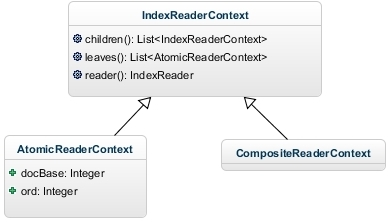
\includegraphics[scale=0.7]{pictures/ReaderContexts.jpg}
 \caption{Struktura kontekstów \texttt{IndexReader}. Źródło: opracowanie własne. \label{fig:indexReaderContexts}}
\end{figure}

Każdy \texttt{IndexReaderContext} potrafi wylistować konteksty readerów potomnych, konteksty liści drzewa readerów oraz wskazać konkretną instancję typu \texttt{IndexReader}, do której jest przypisany. Dodatkowo, konteksty instancji \texttt{AtomicReader} pamiętają wartość \texttt{docBase} -- bazę przenumerowania dokumentów oraz swój numer w wewnętrznej tablicy nadrzędnego \texttt{CompositeReadera} (wartość \texttt{ord}).

\section{Implementacja własnego kodeka}

Format list postingowych jest miejscem, które najprawdopodobniej zmieniłby programista chcący zaimplementować np. nowy algorytm kompresji postingów czy reprezentacji termów. Dlatego zajmiemy się teraz opisem architektury tej części kodeka. 

Jak zostało wspomniane w sekcji \ref{sec:codecStructure}, za format list postingowych odpowiada klasa \texttt{PostingsFormat}. Jej głównym zadaniem jest dostarczenie i zarządzanie cyklem życia dwóch obiektów: \texttt{FieldsProducer} i \texttt{FieldsConsumer}, które są odpowiedzialne za, odpowiednio, odczyt i zapis danych z plików indeksu. Architekturę formatu list postingowych przedstawia rys. \ref{fig:postingFormat}.

\begin{figure}[here]
 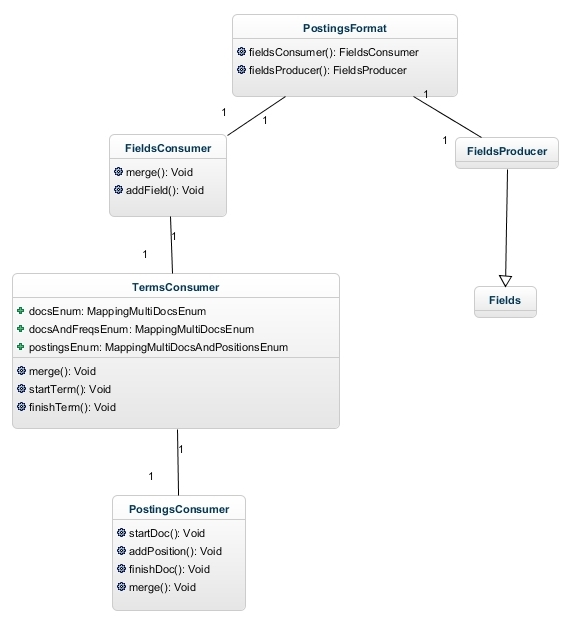
\includegraphics[scale=0.6]{pictures/PostingsFormat.jpg}
 \caption{Schemat klas służących do zapisu formatu list postingowych.\label{fig:postingFormat}}
\end{figure}

Klasa \texttt{FieldsProducer} jest odpowiedzialna za odczyt danych z segmentu -- stąd powiązanie z przedstawioną już wcześniej klasą \texttt{Fields}. \texttt{FieldsConsumer} jest z kolei odpowiedzialny za zapis nowego segmentu (powstałego w wyniku zrzutu danych na dysk lub w wyniku łączenia segmentów). Określenia \emph{producer} i \emph{consumer} mogą wydawać się tutaj mało intuicyjne. Zrozumienie ich ról może ułatwić następujące zdanie: ,,\texttt{FieldsConsumer} \emph{pobiera} (konsumuje) właśnie definiowane pole i zapisuje je w indeksie, podczas gdy \texttt{FieldsProducer} odczytuje pole z indeksu (\emph{produkuje} je z plików indeksu)''.

Dodawanie nowych pól do instancji \texttt{FieldsConsumera} odbywa się za pomocą metody \texttt{addField()} przyjmującej jako parametr obiekt typu \texttt{FieldInfo}, przechowujący informacje o konfiguracji pola (takie jak jego wewnętrzny numer, nazwę, opcje indeksowania, atrybuty, itp.). Metoda ta zwraca obiekt \texttt{TermsConsumer}, pozwalający na dodawanie termów do pola. \texttt{TermsConsumer} posiada trzy atrybuty typu \texttt{DocsEnum} (a konkretniej: typów rozszerzających \texttt{DocsEnum}). Są one wykorzystywane podczas łączenia segmentów -- w zależności od opcji indeksowania, wybierane jest jedno a nich i ono pełni rolę iteratora dokumentów.

Wywołanie \texttt{TermsConsumer.startTerm()} zwraca obiekt \texttt{PostingsConsumer}, który, operując już na numerach dokumentów i pozycjach występowania danego termu, zapisuje listy postingowe.

Oczywiście, wszystkie klasy diagramu \ref{fig:postingFormat} są abstrakcyjne -- wymienione operacje (takie jak dodawanie pola, termu lub dokumentu) muszą być oprogramowane w klasach kodeka. Klasy \texttt{FieldsConsumer}, \texttt{TermsConsumer}, \texttt{PostingsConsumer} posiadają jedynie implementacje metod \texttt{merge()}: według projektantów Lucene łączenie poszczególnych elementów indeksu powinno być niezależne od faktycznego formatu zapisu. Nic jednak nie stoi na przeszkodzie, aby kodek nadpisywał także tę funkcjonalność.

[Tutaj: klasy w obecnym kodeku implementujące te wszystkie funkcjonalności -- opis. Opowiedzenie o tym, że skomplikowanie architektury z rys. \ref{fig:postingFormatRead} i \ref{fig:postingFormatWrite} służy temu, aby można było podmieniać także format słowników termów.]

\begin{figure}[here]
 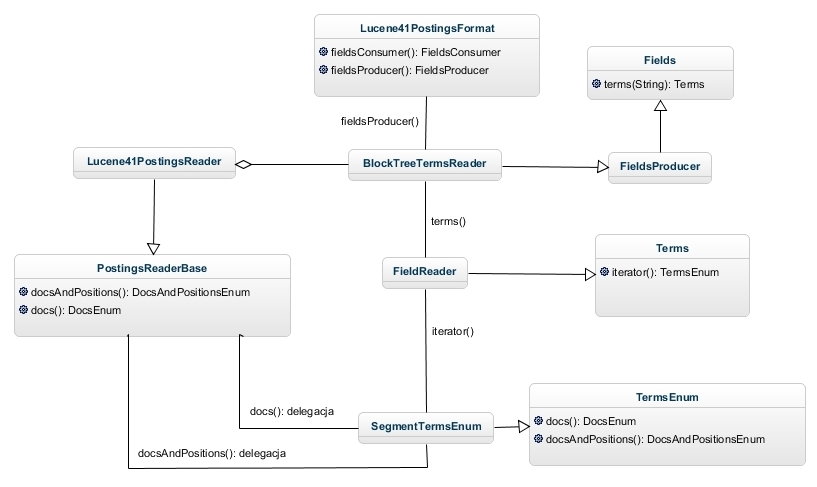
\includegraphics[scale=0.6]{pictures/Lucene41PostingsFormatRead.jpg}
 \caption{Odczyt list postingowych i innych informacji z indeksu odwróconego: schemat klas wykorzystywanych przez domyślny kodek. Źródło: opracowanie własne. \label{fig:postingFormatRead}}
\end{figure}

\begin{figure}[here]
 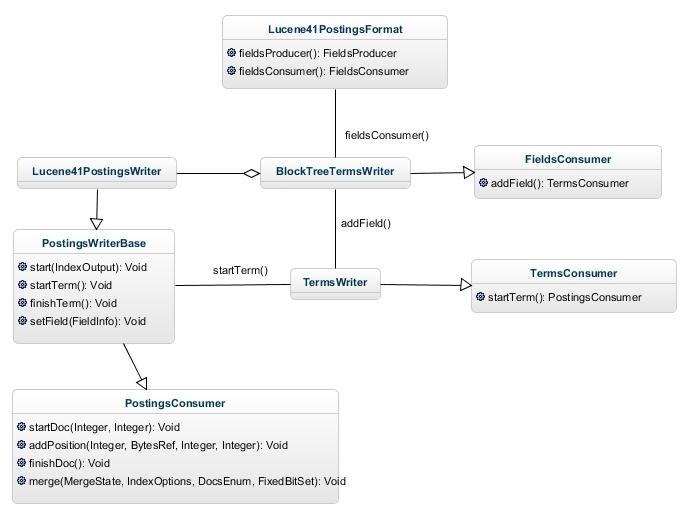
\includegraphics[scale=0.6]{pictures/Lucene41PostingsFormatWrite.jpg}
 \caption{Zapis list postingowych i innych informacji do indeksu odwróconego: schemat klas wykorzystywanych przez domyślny kodek. Źródło: opracowanie własne. \label{fig:postingFormatWrite}}
\end{figure}

\section{Format list postingowych}

W tym podrozdziale opisany zostanie obecnie stosowany format list postingowych (dla domyślnego kodeka używanego w Lucene od wersji 4.1) Schematyczne przedstawienie tego formatu znajduje się na rys. \ref{fig:postingCodingFormat}.

\begin{figure}[here]
 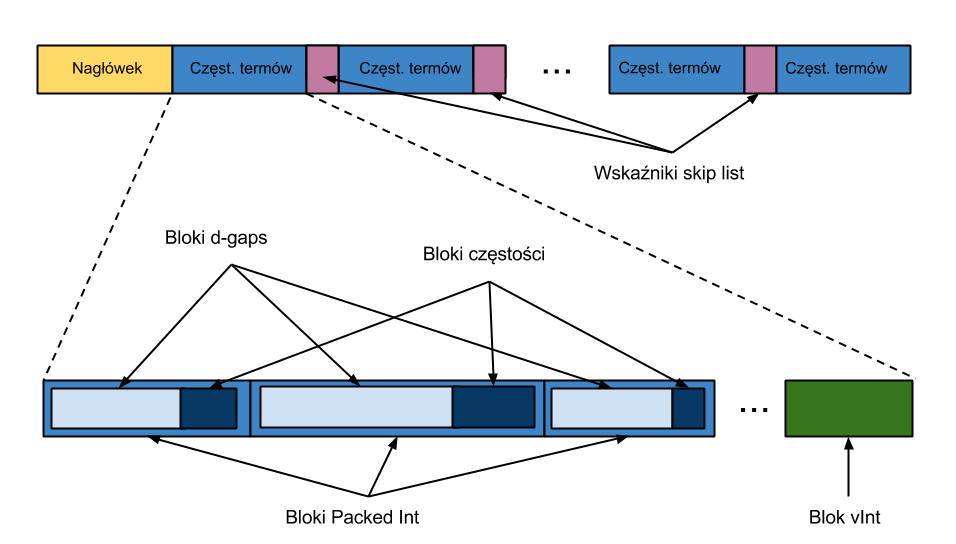
\includegraphics[scale=0.37]{pictures/PostingCodingFormat.png}
 \caption{Schematyczne przedstawienie sposobu zapisu list postingowych. Źródło: opracowanie własne. \label{fig:postingCodingFormat}}
\end{figure}

Elementami list postingowych są różnice pomiędzy numerami dokumentów (zwane dalej \emph{d-gaps} lub \emph{DocDelta}). Na liście postingowej może być dodatkowo przechowywana informacja o liczbe wystąpień danego termu w dokumencie.

Listy postingowe kodowane są blokami dwóch rodzajów. Wszystkie bloki (być może poza ostatnim) są blokami tzw. upakowanymi (\emph{Packed Blocks}). Liczba postingów w takim bloku jest stała i wynosi 128. Jeśli liczba postingów w liście nie jest podzielna przez 128, pozostałe postingi (te, które nie zmieściły się w ostatnim bloku upakowanym) są zapisywane w postaci dodatkowego bloku i są kodowane przy pomocy liczb całkowitych o zmiennej długości (tzw. \emph{vInt format}).

Lista postingowa jest skip listą: istnieje możliwość ,,przeskakiwania'' w niej o całe bloki. Wskaźniki skip list zapisywane są na początku każdego bloku (z wyjątkiem pierwszego).

\subsection{Kodowanie bloków upakowanych}

Każdy blok upakowany (\emph{PackedBlock}) składa się z dwóch części: 
\begin{enumerate}
 \item upakowanych numerów dokumentów (\emph{PackedDocDeltaBlock}, bloki upakowanych \emph{d-gaps}),
 \item (opcjonalnie) części kodującej częstości wystąpienia danego termu w dokumencie (\emph{PackedFreqBlock}, bloki częstości).
\end{enumerate}

Algorytm kodowania numerów dokumentów w bloku upakowanym jest bardzo prosty: najpierw obliczane są różnice pomiędzy kolejnymi numerami dokumentów (tzw. \emph{d-gaps}), a następnie kolejne grupy po 128 postingów są osobno kodowane jako blok upakowany. Dla każdej grupy \emph{d-gaps}, która ma zostać zakodowana jako blok, wybierana jest minimalna liczba bitów, przy pomocy której wszystkie z nich będą mogły zostać przedstawione. Informacja o tej liczbie zapisywana jest w pierwszym bajcie bloku. Następnie zapisywany jest ciąg zakodowanych \emph{d-gaps}.

Dodatkowo, jeśli wszystkie \emph{d-gaps} są takie same (np. jeśli dany term występuje we wszystkich dokumentach i w związku z tym wszystkie \emph{d-gaps} mają wartość 1), w pierwszym bajcie bloku zapisywana jest wartość 0, a następnie -- powtarzająca się liczba jako pojedynczy \texttt{vInt}.

Wedle podobnego schematu kodowana jest część zawierająca częstości wystąpień termu w dokumencie -- z pominięciem obliczania \emph{d-gaps}, które tutaj nie są potrzebne.

\subsection{Kodowanie \texttt{vInt}}

W tym formacie kodowania informacje o numerze dokumentu oraz o częstości występowania termu są zakodowane naprzemiennie (tzn. jeśli częstość występowania termu w danym dokumencie jest większa niż 1, kodowana jest jako kolejna liczba na liście). 

Elementy tego bloku nazywane się \emph{DocDelta} i kodowane są jako liczby \texttt{vInt}. Kodowaniem tym rządzą następujące reguły:
\begin{itemize}
 \item jeśli częstości występowania termu są zaindeksowane, wartość \emph{DocDelta} zawiera informacje zarówno o \emph{d-gap} jak i o częstości,
 \item $\emph{d-gap} = \emph{DocDelta} / 2$ (dzielenie bez reszty)
 \item jeśli $\emph{DocDelta}~\%~2 = 1$, to częstość termu wynosi 1,
 \item jeśli $\emph{DocDelta}~\%~2 = 0$, to częstość występowania termu zakodowana jest jako kolejna liczba (\texttt{vInt}) na liście.
\end{itemize}

Kodowanie liczb \texttt{vInt} (liczb całkowitych o zmiennej długości) odbywa się według podobnego algorytmu, jak opisany w \cite{irbook} w rozdziale 5.3.1 ,,Variable byte encodes''. Pierwszy bit każdego bajtu jest bitem kontynuacji: jeśli jego wartością jest 0, dany bajt jest ostatnim w liczbie. Pozostałe 7 bitów jest faktycznym kodowaniem danej pozycji w liczbie całkowitej: wartości kolejnych bajtów przekładają się na pozycje w systemie o podstawie 128.